\section{Implementation}
\begin{figure}[t!]
    \centering{}
	\subfloat[Architecture] { 
    	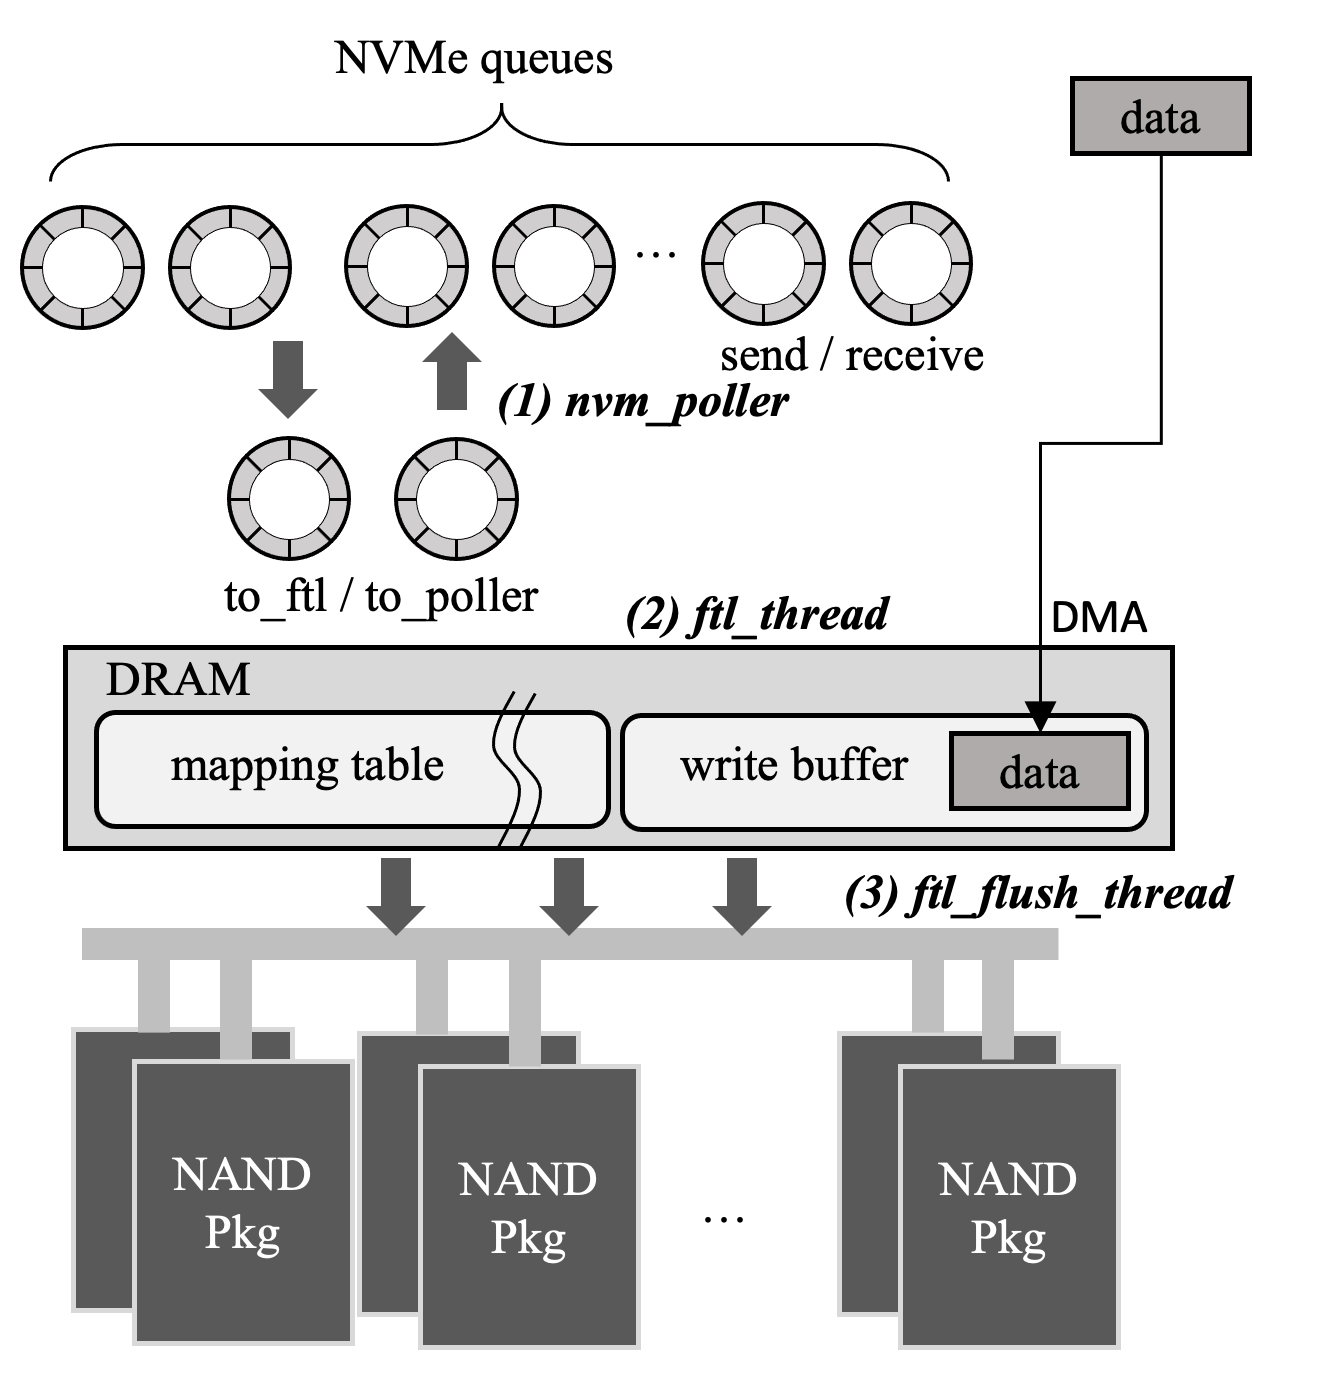
\includegraphics[width=0.3\textwidth]{figure/dawid_ssd_archi_new.eps}
	} \\
	\subfloat[Data structures for FTL]{ 
    	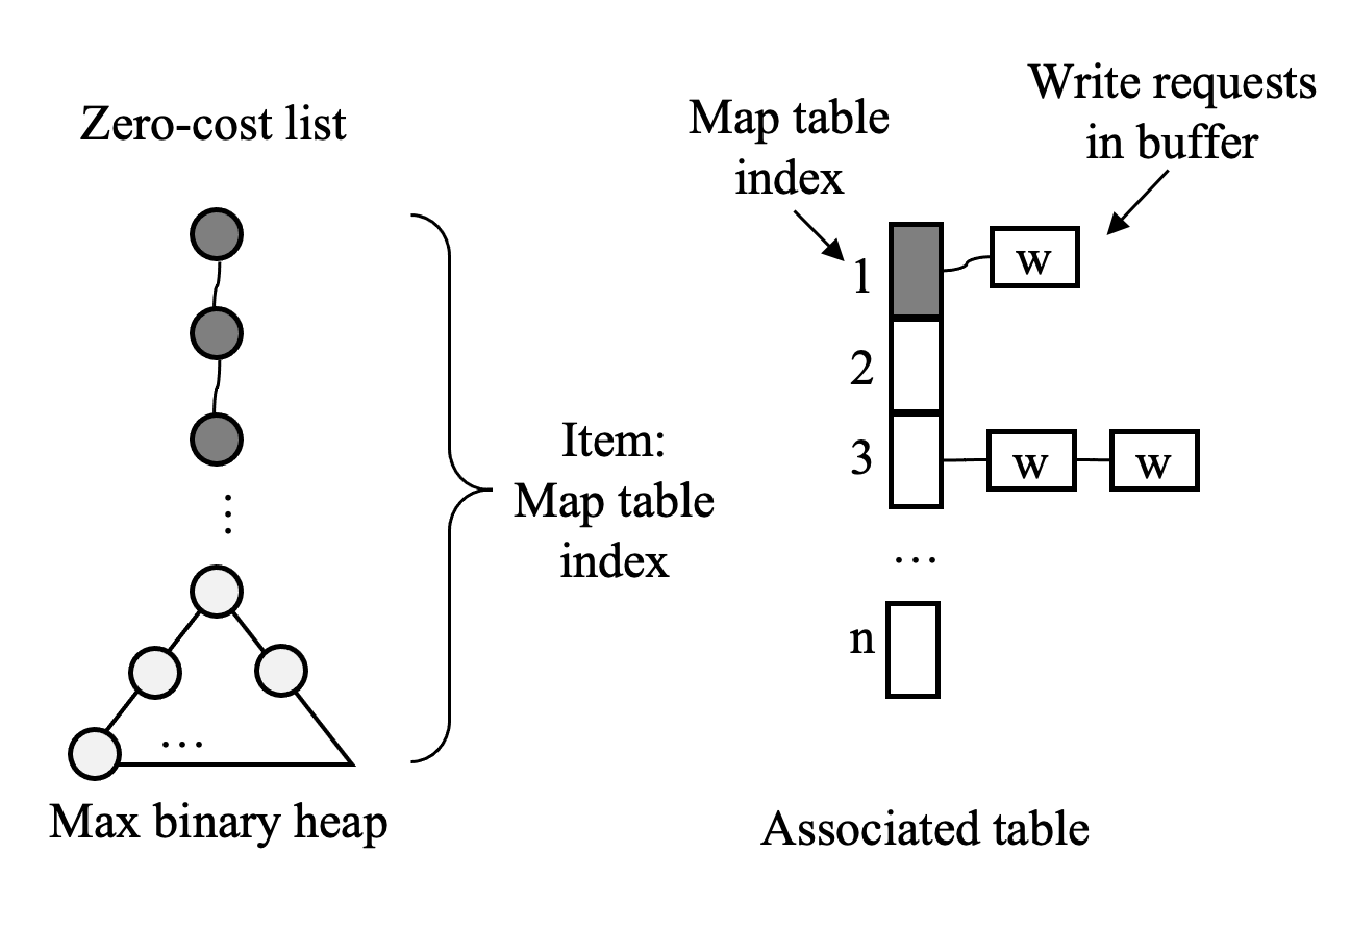
\includegraphics[width=0.4\textwidth]{figure/dawid_ds.eps}
	}

    %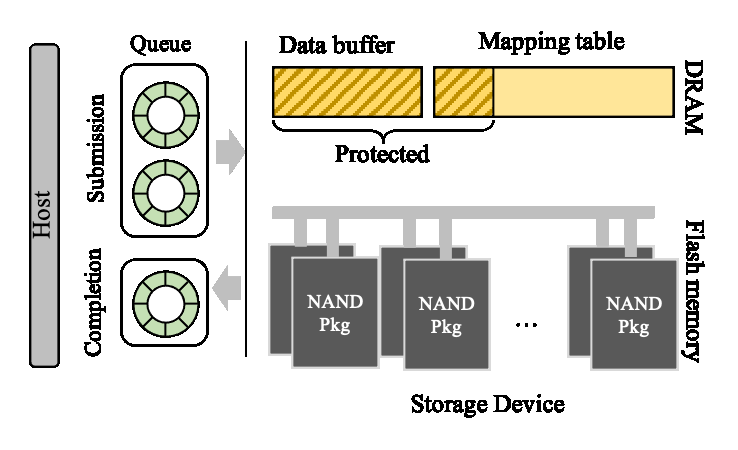
\includegraphics[width=0.4\textwidth]{figure/dawid_ssd_archi.eps}
    \caption{\textbf{Dawid-SSD}}
    \label{fig_dawid_archi}
\end{figure}


\begin{figure*}[!t]
    \centering{}
	\subfloat[Random] { 
	    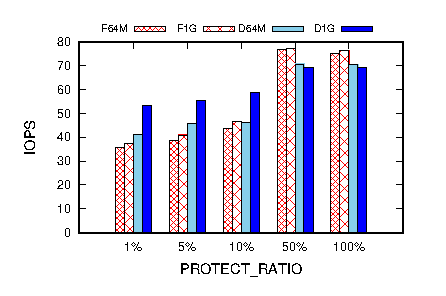
\includegraphics[width=0.3\textwidth]{expr/micro_rslt_220525/perf/perf_RAND.eps}
	} 
	\subfloat[JESD] { 
	    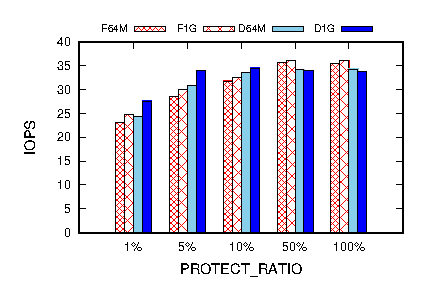
\includegraphics[width=0.3\textwidth]{expr/micro_rslt_220525/perf/perf_JESD.eps}
	}
	\subfloat[TPC-C] { 
	    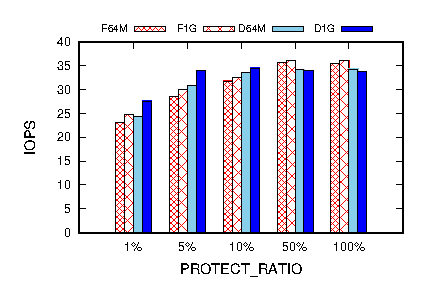
\includegraphics[width=0.3\textwidth]{expr/micro_rslt_220525/perf/perf_JESD.eps}
	}

    \caption{\textbf{IOPS}}
\end{figure*} 


\begin{figure*}[!t]
    \centering{}
	\subfloat[Random] { 
	    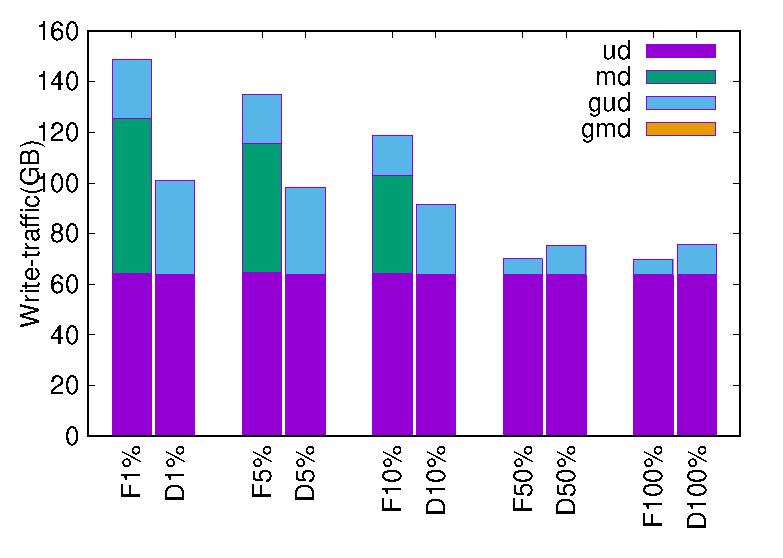
\includegraphics[width=0.3\textwidth]{expr/micro_rslt_220525/wt/RAND_1.eps}
	} 
	\subfloat[JESD] { 
	    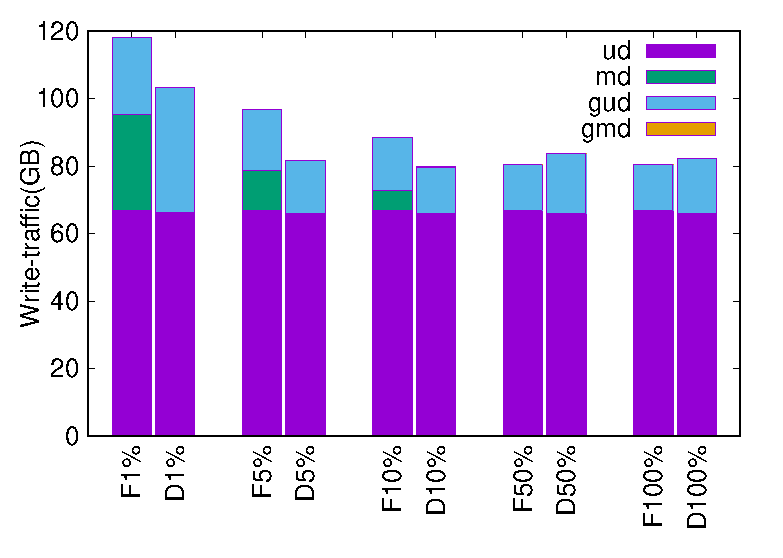
\includegraphics[width=0.3\textwidth]{expr/micro_rslt_220525/wt/JESD_1.eps}
	}
	\subfloat[TPC-C] { 
	    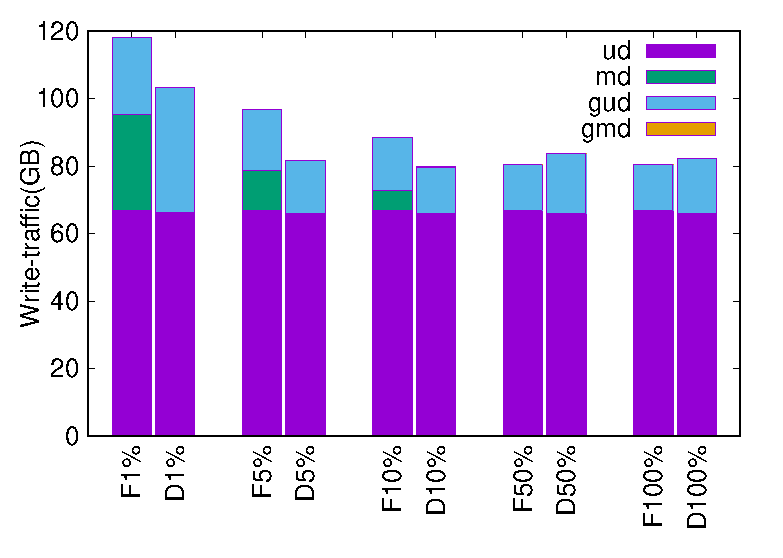
\includegraphics[width=0.3\textwidth]{expr/micro_rslt_220525/wt/JESD_1.eps}
	}
    \caption{\textbf{Write Traffic.}}
\end{figure*} 



We implement \ours{} in \texttt{FEMU}, an open-source SSD development
framework~\cite{li2018case}. Fig.~\ref{fig_dawid_archi} shows the overall
architecture of \ours{}-SSD and its internal data structures. As the original
version of \texttt{FEMU} directly writes data to flash memories without write
buffering, we extend it to use a small-sized write buffer, which aggregates and  
batches user writes into the underlying flash memory.  

\ours{}-SSD maintains three different threads that are executing concrrently
within SSDs.  The \texttt{nvm\_poller} takes a charge of transferring requests
between NVMe queues and FTL-internal queues. The FTL-internal queue consists of
a pair of sub-queues, each of which is named \texttt{to\_ftl} and
\texttt{to\_poller}). This separation is intended to enable a non-blocking
access to queues by allowing only a single writer for each queue.  Second, the
\texttt{ftl\_thread} essentially handles the ingress requests from the internal
queues. For write, it transfers data from the host memory to the SSD-internal
write buffer with DMA and updates the associated entry in a translation page to
point to the write buffer. Then, it notifies the completion of request to the
\texttt{nvm\_poller} by enqueueing the acknowledgement into the
\texttt{to\_poller} queue.  Because \ours{} protects the entire space of write
buffer with capacitance, data persistency is guaranteed for all acknowledged
writes.  For read, the \texttt{ftl\_thread} retrieves the requested data by
consulting the mapping table and transfers it to the host. 

The \texttt{ftl\_flush\_thread} plays a role of writing data from a DRAM-buffer
into a flash memory.  With the \texttt{FIFO} policy, the user writes are issued
to NAND flash memory in the order they arrive into the buffer. However, \ours{}
flushes buffered writes in the order such that it least increases the dirty memory
footprint of the mapping table.  To realize this design, \ours{} maintains two
data structures, as depicted in Fig.~\ref{fig_dawid_archi}(b). First, \textit{a
zero-cost list} that holds the indexes to tranlsation pages that is already
in a dirty state, and second, \textit{a max binary heap} that
maintains the indexes to translation pages sorted by the number of buffered
user write requests associated with that page.  

%When there is sufficient bandwidth at underlying NAND flash subsystem for writes, 
When a half of the write buffer becomes occupied, flushing is invoked. \ours{}-SSD
first flushes user data whose translation pages in the zero-cost list, and then
persists user data as their translation pages are ordered by the max binary
heap. By doing so, each user write minimizes the number of eventual
translation page write, and each translation page write maximizes the number of
persisted mapping entries. These data structures are updated by the \texttt{ftl\_thread} 
when a write request arrives at SSD. 
To exploit the SSD internal parallelism, we send data to flash memory in
batches by the number of NAND flash chips that can be written simultaneously.

Once the write operations of NAND flash memory complete,
\texttt{ftl\_flush\_thread} updates the mapping table entries to point to the
physical address of the data in a flash memory.  At this moment, if the number
of dirty mapping table pages goes beyond the protectable number of pages,
\texttt{ftl\_flush\_thread} persists the mapping table page to flash memory.
This is also conducted in batches by the number of NAND flash chips that can be
written in parallel.


\section{Evaluation}
%We assume 1\% of the mapping table is protected via capacitors in a 64GB SSD. 
%The 64GB SSD is using DRAM and assumes that 1\% of the mapping table is
%protected. 
We perform the experiments on a machine with a 20-core Intel Xeon(R) Silver
4114 CPU running at 2.2GHz and 84GB memory. We run FEMU (QEMU-based SSD
emulator) configured to use 10 cores, 4GB DRAM for main memory, and 16GB DRAM
for SSD emulation. The SSD maintains a mapping table entirely in DRAM partially 
protected with capacitance.

We measure the average IOPS and write traffic varying the protected ratio of
the mapping table from 1\% to 100\%. We study two different size of write
buffers, which are 64MB and 1GB, respectively. 
We use two benchmarks for \ours{} performance evaluation. Using the fio
benchmark~\cite{fio-bench}, we generate two kinds of workloads: the 4KB of
random writes (denoted as RANDOM) and the skewed read-write mixed workload that follows JESD219 (JESD)
using 8 threads.  A total of 90GB of data was written to the 30GB area.



%\begin{figure*}[t]
%    \centering{}
%	\subfloat[OLTP] { 
%	    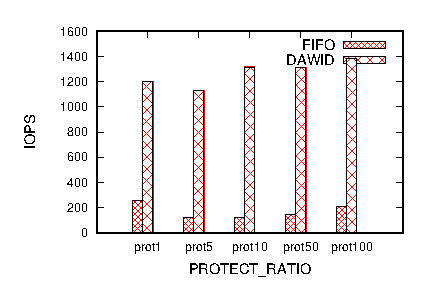
\includegraphics[width=0.3\textwidth]{expr/macro_220517/perf/OLTP/perf_OLTP.eps}
%	} 
%	\subfloat[Write Traffic] { 
%	    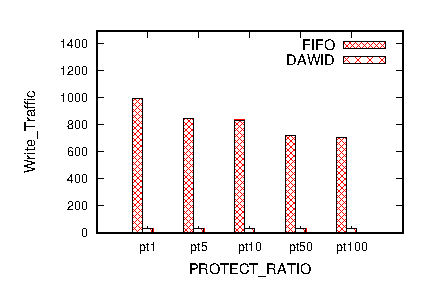
\includegraphics[width=0.3\textwidth]{expr/macro_220517/wt/OLTP/perf_OLTP.eps}
%	} 
%    \caption{\textbf{OLTP}}
%\end{figure*} 



%\begin{figure*}[t]
%    \centering{}
%	\subfloat[Sequential] { 
%	    %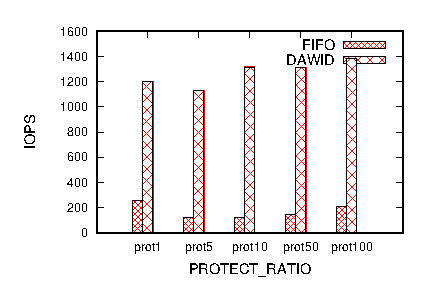
\includegraphics[width=0.3\textwidth]{expr/macro_220517/perf/OLTP/perf_OLTP.eps}
%	    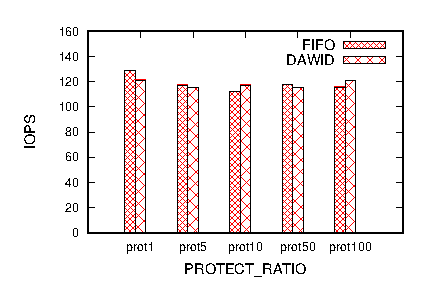
\includegraphics[width=0.3\textwidth]{expr/micro_220517/perf/SEQ/perf_SEQ.eps}
%	} 
%	\subfloat[Random] { 
%	    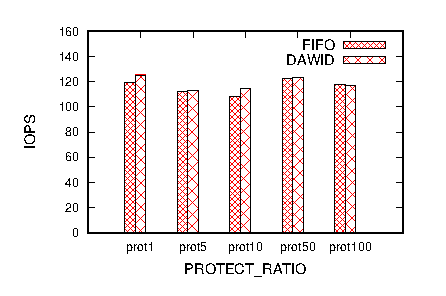
\includegraphics[width=0.3\textwidth]{expr/micro_220517/perf/RAND/perf_RAND.eps}
%	} 
%	\subfloat[JESD] { 
%	    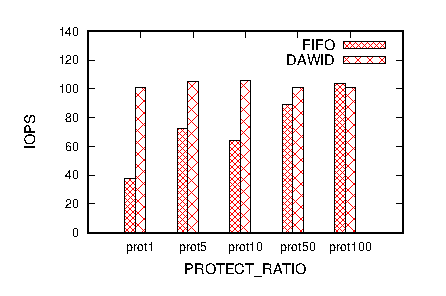
\includegraphics[width=0.3\textwidth]{expr/micro_220517/perf/JESD/perf_JESD.eps}
%	}
%    \caption{\textbf{IOPS}}
%\end{figure*} 
%



